\documentclass[xcolor=dvipsnames,mathserif,9pt]{beamer} %handout
%\usefonttheme{serif}%{structurebold}%{structuresmallcapsserif}%{serif}

\usepackage{graphicx}
\usepackage{amsmath}
\usepackage{amssymb}
\usepackage[font=footnotesize]{caption} % set the captain font size to 8 (i.e. footnotesize)
\usepackage{subfig} % uses subfloats within a single float MUST after the package {caption}!!
\usepackage{natbib}
%\usepackage{cite} % sort the reference in the article by number or alphabatic
\usepackage{color}
\usepackage{algorithm} % options: boxed [section]
\usepackage{algpseudocode} % for algorithm
%\usepackage{enumerate}
\usepackage{enumitem} % directly use itemize, easily specify indent and everything
\setlist[itemize]{leftmargin=*,label=$\bullet$}%leftmargin=*,itemsep=0pt} %topsep=5pt
\setlist[enumerate]{label={\arabic*)}}
\usepackage{hyperref}
\usepackage{wrapfig}
\usepackage{textpos}
\usepackage{bibentry} % for publication list
\makeatletter\let\saved@bibitem\@bibitem\makeatother % make hyperref and bibentry compatible!!!
\nobibliography*
\usepackage{fancybox}% shadow for image
%\usepackage{empheq} % emphasize equations
\usepackage{bm}
\usepackage{arydshln} % for dashline in table or matrix
\linespread{1.3}
\usepackage{multimedia}

\usepackage{setspace} \setstretch{1.2}

\usepackage{framed}
\colorlet{shadecolor}{black!5}
% for box, page breakable, very good!!
\usepackage[framemethod=TikZ]{mdframed}%
\mdfdefinestyle{myFrame}{%
    linecolor=gray!15!white,%gray
    outerlinewidth=0.1pt,
    roundcorner=3pt,
    skipabove=15pt, % the space before the entire box
    skipbelow=15pt, % the space after the entire box. Please see the figure 2 in the manual, very clear!
    innertopmargin=10pt,%\baselineskip,
    innerbottommargin=10pt,%\baselineskip,
    %innerrightmargin=10pt,
    %innerleftmargin=10pt,
    splittopskip=\baselineskip,
    splitbottomskip=\baselineskip,
    backgroundcolor=gray!10!white,
    frametitlerule=true,
    frametitlebackgroundcolor=gray!20!white,
    frametitleaboveskip=5pt,
    frametitlebelowskip=5pt,
}
\mdfdefinestyle{myAlgo}{%
    linecolor=gray!100!white,%gray
    outerlinewidth=0.1pt,
    roundcorner=3pt,
    skipabove=15pt, % the space before the entire box
    skipbelow=15pt, % the space after the entire box. Please see the figure 2 in the manual, very clear!
    innertopmargin=10pt,%\baselineskip,
    innerbottommargin=10pt,%\baselineskip,
    %innerrightmargin=10pt,
    %innerleftmargin=10pt,
    splittopskip=\baselineskip,
    splitbottomskip=\baselineskip,
    backgroundcolor=gray!0!white,
    frametitlerule=true,
    frametitlebackgroundcolor=gray!20!white,
    frametitleaboveskip=5pt,
    frametitlebelowskip=5pt,
}


\usepackage{tikz}
\usetikzlibrary{calc} % for calculation functions in Tikz let, in commands in Tikz
\usetikzlibrary{shapes} % for block diagram
\usetikzlibrary{chains}
\usetikzlibrary{fit}
\usetikzlibrary{arrows}
\usetikzlibrary{decorations.text} % text along path

\newcommand{\blue}[1]{\textcolor{blue}{#1}}
\definecolor{myred}{RGB}{200,0,0}
\newcommand{\red}[1]{\textcolor{myred}{#1}} %magenta purple
\newcommand{\I}{\mathcal{I}}
\newcommand{\tr}{\mathrm{tr}}
\newcommand{\Null}{\mathrm{Null}}
\newcommand{\Range}{\mathrm{Range}}
\newcommand{\one}{\mathbf{1}}
\newcommand{\rank}{\mathrm{rank}}
\newcommand{\myspan}{\mathrm{span}}
\newcommand{\mydiag}{\mathrm{diag}}
\newcommand{\D}{\mathrm{d}}
\renewcommand{\d}{\mathrm{d}}
\newcommand{\blkdiag}{\mathrm{blkdiag}}
\newcommand{\sgn}{\mathrm{sgn}}
\newcommand{\T}{\mathrm{T}}
\newcommand{\myqed}{\hfill$\blacksquare$}
\newcommand{\ep}{\varepsilon}
\newcommand{\sig}{\mathrm{sig}_a}
%\newcommand{\sigep_}[1]{\sig(\ep_{#1})}
\newcommand{\R}{\mathbb{R}}
\newcommand{\A}{\mathcal{A}}
\newcommand{\G}{\mathcal{G}}
\newcommand{\E}{\mathbb{E}}
\newcommand{\X}{\mathcal{X}}
\newcommand{\V}{\mathcal{V}}
\newcommand{\N}{\mathcal{N}}
\newcommand{\M}{\mathcal{M}}
\renewcommand{\H}{\mathcal{H}}
\renewcommand{\L}{\mathcal{B}}
\renewcommand{\S}{\mathcal{S}}
\newcommand{\xe}{x_{\text{e}}}
%\newcommand{\Null}[1]{\mathrm{Null}\left(#1\right)}
\newcommand{\sk}[1]{\left[#1\right]_\times} % skew symmetric operator
\newcommand{\dia}[1]{\mathrm{diag}\left(#1\right)} % block diagnal matrix
%\renewcommand{\span}[1]{\mathrm{span}\left\{#1\right\}} % ERROR when redefine \span
\newcommand{\Var}{\mathrm{Var}}
\newcommand{\var}{\mathrm{var}}


\graphicspath{{figures/}}

% for tikz, theorem, lemma ... environments have already been declared. You don't need to declare, or you need to use other names than theorem or lemma, such as my_theorem.
%\newtheorem{my_theorem}{Theorem}
%\newtheorem{my_lemma}{Lemma}
\newtheorem{assumption}{Assumption} % necessary for beamer
%\newtheorem{my_remark}{Remark}
\newtheorem{proposition}{Proposition} % necessary for beamer
%\newtheorem{my_corollary}{Corollary}
%\newtheorem{my_example}{Example}
%\newtheorem{my_definition}{Definition}
%\newtheorem{my_problem}{Problem}

%##################################################
\newcommand{\pagetitle}[1]{\textbf{\textcolor{BlueViolet}{$\circ$ #1}}} %!!!
\newcommand{\pagehighlight}[1]{\textbf{\textcolor{Brown}{#1}}} %!!!
\newcommand{\mypause}{\pause} % this is useful for slide show. if you don't want pause any more, just set it as blank
%\newcommand{\mybullet}{\textcolor{BlueViolet}{$\blacksquare$} }%{$\rhd$ }
%\newcommand{\myhighsign}{$\star$ }% the sign to highlight a sentence

%##################################################
% To highlight equation. Example: \begin{align*} \boxed{xxx} \end{align*}
% does not support multiline equations
% put color to \boxed math command
\newcommand*{\boxcolor}{gray}
\makeatletter
\renewcommand{\boxed}[1]{\textcolor{\boxcolor}{%
%\tikz[baseline={([yshift=-1ex]current bounding box.center)}] \node [rectangle, minimum width=1ex,rounded corners,draw] {\normalcolor\m@th$\displaystyle#1$};}}
\tikz[baseline={([yshift=-1ex]current bounding box.center)}] \node [rectangle, minimum width=2ex,rounded corners,draw] {\normalcolor\m@th$\displaystyle#1$};}}
\makeatother

%##################################################
% set my own theme
\def\structureHeight{9mm}
\usetheme[height=\structureHeight]{Rochester}
\usecolortheme[RGB={0,0,128}]{structure}
\setbeamertemplate{items}[circle]%rectangle, triangle,circle
\setbeamertemplate{blocks}[rounded][shadow=true]
\setbeamertemplate{navigation symbols}{}
%\addtobeamertemplate{frametitle}{} % specify the logo
%{
%    \begin{textblock*}{100mm}(.87\textwidth,-\structureHeight)
%        \includegraphics[height=6.6mm,width=3cm,keepaspectratio]{../common_figures_private/westlake_logo.png} % add logo
%    \end{textblock*}
%}
\addtobeamertemplate{frametitle}{\vskip4pt}{} % specify
%\setbeamerfont{frametitle}{size=\large}
\definecolor{mylightgray}{RGB}{240 240 240}
\definecolor{mykhaki}{RGB}{240 230 140}% khaki color
\definecolor{mylightYellow}{RGB}{255,255,224} % light yellow
%\setbeamercolor{beamercolor1}{bg=mylightgray, fg=black}
%\setbeamercolor{beamercolor2}{bg=mylightYellow,fg=black}%{bg=yellow!90!white, fg=black}
% background and foreground color
\setbeamercolor{background canvas}{bg=black!0!white} % background color of every slide! My previous value was black!10!white for my lecture videos!
\setbeamercolor{normal text}{bg=black!10!white} % background color for e.g. theorem environment. When canvas is 10, here it can be 20; the bg for normal text changes the color of hidden text when you use overlay

\setbeamercolor{block title}{bg=mykhaki,fg=black}
\defbeamertemplate{footline}{zsy_frameNumber}
{%
  \hspace{5pt}  \emph{Shiyu Zhao}
  \hspace*{\fill}%
  \usebeamercolor[fg]{page number in head/foot}%
  \insertframenumber\,/\,\inserttotalframenumber \vspace{0pt} \hspace{5pt}
  \vskip5pt
}
\setbeamertemplate{footline}[zsy_frameNumber]
%##################################################
\setbeamercovered{transparent=0} % a good value for transparent text is 20
% when using the overlay commands like \onslide or \uncover, the text will NOT be invisible, instead it will be like transparent
%\pause will also have the transparent effect: command \pause is easy to use: to make it invisible, change the value to zero.



\usepackage{multimedia}

%\newcommand{\blue}[1]{\textcolor{blue}{#1}}
%\newcommand{\red}[1]{\textcolor{red}{#1}}
%\newcommand{\I}{\mathcal{I}}
\begin{document}

%%%%%%%%%%%%%%%%%%%%%%%%%%%%%%%%%%%%%%%%%%%%%%%%%%%%%%%%%%%%%%%%%%%%%%%%%%%%%%%%%
% define the author, date etc. information
%\subtitle{Mathematical and Biological Foundation for Reinforcement Learning}
\title{Lecture 2: State Value and Bellman Equation}

\author{Shiyu Zhao
\newline
\newline {\small Department of Artificial Intelligence}
\newline {\small Westlake University}
}
%\logo{\includegraphics[width=1cm,height=1cm,keepaspectratio]{NUSLogo.png}~}
%\date{\today}
\date{}
\subject{}


%%%%%%%%%%%%%%%%%%%%%%%%%%%%%%%%%%%%%%%%%%%%%%%%%%%%%%%%%%%%%%%%%%%%%%%%%%%%%%%%%

{
\setbeamertemplate{footline}{} % remove the frame number of the title page
\begin{frame}
    %\frametitle{Lecture: Networked Dynamic Systems}
    \addtocounter{framenumber}{-1} % discounter the title page, otherwise the frame number starts from 2 instead of 1
    \titlepage % this only gives the author etc. information
\end{frame}
}


\begin{frame}
\frametitle{Outline}
\begin{figure}[h]
  \centering
\includegraphics[width=0.8\linewidth]{Figure_chapterRelationship.pdf}
\end{figure}
\end{frame}
%---------------------
\begin{frame}
\frametitle{Outline}
\tableofcontents
\end{frame}
\AtBeginSection[]% put it to the start of each section
{
  \begin{frame}
    \frametitle{Outline}
    \tableofcontents[currentsection]
  \end{frame}
}
%--------------------------------------
\AtBeginSection[]% put it to the start of each section
{
  \begin{frame}
    \frametitle{Outline}
    \tableofcontents[currentsection]
  \end{frame}
}
\section{Motivating examples: from table to function}
%-----------------------------
\begin{frame}
\frametitle{Motivating examples: from table to function}

So far in this book, state and action values are represented by \blue{tables}.

\pause
\begin{itemize}
\item For example, state value:
\end{itemize}
{\footnotesize
\begin{table}[th!]
\centering
%\resizebox{\columnwidth}{!}{
\begin{tabular}{c|c|c|c|c}%{|p{1.5cm}|p{1.5cm}|p{1.5cm}|p{1.5cm}|p{1.5cm}|}%{|p{0.45\textwidth}|p{0.45\textwidth}|}
  % after \\: \hline or \cline{col1-col2} \cline{col3-col4} ...
  \hline
  \,\,{State}\,\, & $s_1$ & $s_2$ & $\cdots$ & $s_n$\\
  \hline
  \,\,{Value}\,\, & $\quad v_{\pi}(s_1)\quad$ & $\quad v_{\pi}(s_2)\quad $ & $\quad \cdots\quad $ & $\quad v_{\pi}(s_n)\quad $\\
  %\hline
  %\,\,{Estimated value}\,\, & $\quad \hat{v}(s_1)\quad$ & $\quad \hat{v}(s_2)\quad $ & $\quad \cdots\quad $ & $\quad \hat{v}(s_n)\quad $\\
  \hline
\end{tabular}
\label{table_compareTDMC}
\end{table}
}

\pause
\begin{itemize}
\item For example, action value:
\end{itemize}
{\scriptsize
\begin{table}[h!]
\centering
%\resizebox{\columnwidth}{!}{
\begin{tabular}{c|c|c|c|c|c}
  % after \\: \hline or \cline{col1-col2} \cline{col3-col4} ...
  \hline
   & \blue{$a_1$} & \blue{$a_2$} & \blue{$a_3$} & \blue{$a_4$} & \blue{$a_5$} \\
  \hline
  \blue{$s_1$} & $q_\pi(s_1,a_1)$ & $q_\pi(s_1,a_2)$ & $q_\pi(s_1,a_3)$ & $q_\pi(s_1,a_4)$ & $q_\pi(s_1,a_5)$ \\
  \hline
  \vdots & \vdots & \vdots & \vdots & \vdots & \vdots \\
  \hline
  \blue{$s_9$} & $q_\pi(s_9,a_1)$ & $q_\pi(s_9,a_2)$ & $q_\pi(s_9,a_3)$ & $q_\pi(s_9,a_4)$ & $q_\pi(s_9,a_5)$ \\
  \hline
\end{tabular}
%}
\end{table}
}
\pause
\begin{itemize}
\item \blue{Advantage}: intuitive and easy to analyze
\pause
\item \blue{Disadvantage}: difficult to handle \red{large or continuous }state or action spaces. Two aspects: 1) storage; 2) generalization ability
\end{itemize}
\end{frame}
%---------------------
\begin{frame}
\frametitle{Motivating examples: from table to function}

Consider an example:
\begin{itemize}
\item There are $n$ states: $s_1,\dots,s_n$.

\item The state values are $v_\pi(s_1),\dots,v_\pi(s_n)$, where $\pi$ is a given policy.

\item $n$ is very large!

\item We hope to use a simple curve to approximate these values.
\end{itemize}

\end{frame}
%---------------------
\begin{frame}
\frametitle{Motivating examples: from table to function}
For example, we can use a simple \blue{straight line} to fit the dots.

\begin{figure}[h]
\centering
\includegraphics[width=0.5\linewidth]{chapterFA_fig_curveFitting}
%\caption{An illustration of function approximation of samples.}
%\label{chapterFA_illustrateFA}
\end{figure}

\pause
Suppose the equation of the straight line is
\begin{align*}%\label{chapterFA_eq_demoCurveFitting}
\hat{v}(s,w)=as+b
\onslide<3->{=\underbrace{[s,1]}_{\phi^T(s)}
\underbrace{\left[
  \begin{array}{c}
    a \\
    b \\
  \end{array}
\right]}_{w}=\phi^T(s)w}
\end{align*}
\onslide<4->{
$w$ is the \blue{parameter vector}; $\phi(s)$ the \blue{feature vector} of $s$; $\hat{v}(s,w)$ is \blue{linear} in $w$.
}

\end{frame}
%---------------------
\begin{frame}
\frametitle{Motivating examples: from table to function}
Difference between the tabular and function methods:

\vspace{10pt}
\textbf{Difference 1: How to \emph{retrieve} the value of a state}
\begin{itemize}
\pause
\item
When the values are \red{represented by a table}, we can directly read the value in the table.
\pause
\item
When the values are \red{represented by a function}, we need to input the state index $s$ into the function and calculate the function value.
\visible<4->{
\begin{figure}[h]
  \centering
  \includegraphics[width=0.33\linewidth]{chapterFA_fig_vhatsw}
  %\caption{An illustration of the process for retrieving the value of $s$ when using the function approximation method.}
  %\label{chapterFA_fig_vhatsw}
\end{figure}}
\pause\pause
For example, $s\rightarrow\phi(s)\rightarrow \phi^T(s)w=\hat{v}(s,w)$
\pause
\begin{itemize}
\item[-]
\blue{Benefit: storage. We do not need to store $|\S|$ state values. We only need to store a lower-dimensional $w$.}
\end{itemize}
\end{itemize}

\end{frame}
%---------------------
\begin{frame}
\frametitle{Motivating examples: from table to function}
Difference between the tabular and function methods:

\vspace{10pt}
\textbf{Difference 2: How to \emph{update} the value of a state}
\begin{itemize}
\pause
\item When the values are \red{represented by a table}, we can \blue{directly} rewrite the value in the table.

\pause
\item
When the values are \red{represented by a function}, we must update $w$ to change the values \blue{indirectly}.

\pause
\begin{itemize}
\item[-] How to update $w$ will be addressed in detail later.
\end{itemize}
\end{itemize}
\end{frame}
%---------------------
\begin{frame}
\frametitle{Motivating examples: from table to function}
Difference between the tabular and function methods:

\vspace{5pt}
\textbf{Difference 2: How to \emph{update} the value of a state}
\vspace{-15pt}
\begin{figure}[h]
  \centering
  \subfloat[Tabular method%: when $\hat{v}(s_2)$ is updated, the other values remain the same.
  ]{\includegraphics[width=0.9\linewidth]{chapterFA_fig_generalizationAbility1}}\\
  \vspace{-5pt}
  \subfloat[Function method%: when we update $\hat{v}(s_2)$ by changing $w$, the values of the neighboring states are also changed.
  ]{\includegraphics[width=0.9\linewidth]{chapterFA_fig_generalizationAbility2}}
  %\caption{An illustration of how to update the value of a state.}
  %\label{chapterFA_fig_generalizationAbility}
\end{figure}

\pause
\setcounter{subfigure}{0}
\blue{\textbf{Benefit: generalization ability.} When we update $\hat{v}(s,w)$ by changing $w$, the values of the neighboring states are also changed.}
\end{frame}
%---------------------
\begin{frame}
\frametitle{Motivating examples: from table to function}

The benefits are \blue{not free}. It comes with a \blue{cost}: the state values can not be represented accurately. This is why this method is called \blue{approximation}.

\vspace{5pt}
\pause
We can fit the points more precisely using \blue{high-order curves}:

\vspace{-10pt}
\pause
\begin{align*}
\hat{v}(s,w)= as^2+bs+c
=\underbrace{[s^2,s,1]}_{\phi^T(s)}
\underbrace{\left[
  \begin{array}{c}
    a \\
    b \\
    c \\
  \end{array}
\right]}_{w}=\phi^T(s)w.
\end{align*}

\pause
In this case,
\begin{itemize}
\item The dimensions of $w$ and $\phi(s)$ increase; the values may be fitted more accurately.
\item Although $\hat{v}(s,w)$ is \blue{nonlinear in $s$}, it is \blue{linear in $w$}. The nonlinearity is contained in $\phi(s)$.
\end{itemize}

\end{frame}
%----------------------
\begin{frame}
\frametitle{Motivating examples: from table to function}

Quick summary:
\begin{itemize}
\item \textbf{Idea:} Approximate the state and action values using \blue{parameterized functions}:
    $\hat{v}(s,w)\approx v_\pi(s)$ where $w\in\R^m$ is the parameter vector.
\pause
\item \textbf{Key difference:} How to retrieve and change the value of $v(s)$
\pause
\item \textbf{Advantages:}
\begin{enumerate}
\item \textbf{Storage:} The dimension of $w$ may be much smaller than $|\S|$.
\pause
\item \textbf{Generalization:} When a state $s$ is visited, the parameter $w$ is updated so that the values of some other unvisited states can also be updated.
\end{enumerate}
\end{itemize}
\end{frame}
%%---------------------
%\begin{frame}
%\frametitle{Motivating examples: from table to function}
%
%\textbf{Questions: }
%What feature vector should we use to fit the data points? Should we fit the points as a first-order straight line or a second-order curve?
%
%\pause
%The answer is nontrivial.
%\begin{itemize}
%\item That is because the selection of feature vector relies on certain domain knowledge. The better we understand a problem, the better feature vectors we can select.
%
%\pause
%\item If we do not have domain knowledge, a popular solution is to use neural networks to let the network learn features and then fit the points automatically.
%\end{itemize}
%
%\end{frame}
%%---------------------
%\begin{frame}
%\frametitle{Motivating examples: from table to function}
%
%\textbf{Question: }How to find the optimal parameter vector?
%
%\pause
%\textbf{Answer: }This is a regression problem. We can find the optimal $w$ by optimizing the following objective function:
%\pause
%\begin{align*}
%J_1=\sum_{i=1}^{|\S|} \|\phi^T(s_i)w-v_\pi(s_i)\|^2
%&=
%\left\|
%\left[
%    \begin{array}{c}
%      \phi^T(s_1) \\
%      \vdots \\
%      \phi^T(s_{|\S|}) \\
%    \end{array}
%  \right]w
%-
%\left[
%    \begin{array}{c}
%      v_\pi(s_1)\\
%      \vdots \\
%      v_\pi(s_{|\S|})\\
%    \end{array}
%  \right]
%\right\|^2\\
%&\doteq \|\Phi w-v_\pi\|^2,
%\end{align*}
%where $\Phi\in\R^{{|\S|}\times 2}$ and $v_\pi\in\R^{|\S|}$.
%
%\pause
%The optimal value of $w$ that can minimize $J_1$ can be obtained as
%$$w^*=(\Phi^T\Phi)^{-1}\Phi v_\pi.$$
%
%Exercise: Solve this least-squares problem and verify that $w^*$ is the solution.
%
%\end{frame}
%--------------------------------------
\AtBeginSection[]% put it to the start of each section
{
  \begin{frame}
    \frametitle{Outline}
    \tableofcontents[currentsection]
  \end{frame}
}
\section{Algorithm for state value estimation}
%---------------------
\subsection{Objective function}
\begin{frame}
 \frametitle{Outline}
 \tableofcontents[currentsection]
\end{frame}
%---------------------
\begin{frame}
\frametitle{Objective function}
Introduce in a more formal way:
\begin{itemize}
\pause
\item Let $v_\pi(s)$ and $\hat{v}(s,w)$ be the \blue{true state value} and the \blue{estimated state value}, respectively.
\pause
\item Our goal is to find an \blue{optimal $w$} so that $\hat{v}(s,w)$ can best approximate $v_\pi(s)$ for every $s$.
\pause
\item This is a \blue{policy evaluation problem}. Later we will extend to policy improvement.
\end{itemize}

\vspace{5pt}
\pause
To find the optimal $w$, we need \blue{two steps}.
\begin{itemize}
\pause
\item The first step is to define an objective function.
\pause
\item The second step is to derive algorithms for optimizing the objective function.
\end{itemize}
\end{frame}
%---------------------
\begin{frame}
\frametitle{Objective function}
The \textbf{objective function} is
\begin{align*}%\label{chapterFA_eq_objFunctionforFA}
J(w)=\E[(v_\pi(S)-\hat{v}(S,w))^2].
\end{align*}
\begin{itemize}
\pause
\item
\blue{Our goal} is to find the best $w$ that can minimize $J(w)$.
\pause
\item
The expectation is with respect to the random variable $S\in\S$.

\red{What is the probability distribution of $S$?}
\begin{itemize}
\pause
\item[-]
This is new. We have not discussed the probability distribution of states so far.
\pause
\item[-]
There are several ways to define the probability distribution of $S$.
\end{itemize}

\end{itemize}
\end{frame}
%---------------------
\begin{frame}
\frametitle{Objective function}
\textbf{The first way is to use a \blue{uniform distribution}.}
\begin{itemize}
\pause
\item
That is to treat all the states to be \blue{equally important} by setting the probability of each state as $1/|\S|$.
\pause
\item
In this case, the objective function becomes
\begin{align*}
J(w)=\E[(v_\pi(S)-\hat{v}(S,w))^2]=\frac{1}{|\S|}\sum_{s\in\S}(v_\pi(s)-\hat{v}(s,w))^2.
\end{align*}

\pause
\item
\textbf{Drawback:}
\begin{itemize}
\item[-] \blue{The states may not be equally important.} For example, some states may be rarely visited by a policy. Hence, this way does not consider the real dynamics of the Markov process under the given policy.
\end{itemize}
\end{itemize}
\end{frame}
%---------------------
\begin{frame}
\frametitle{Objective function}
\textbf{The second way is to use the \blue{stationary distribution}.
}
\pause
\begin{itemize}
\item
Stationary distribution is an important concept that will be frequently used in this course. It describes the \blue{long-run behavior} of a Markov process.
\pause
\item
Let \red{$\{d_\pi(s)\}_{s\in\S}$} denote the stationary distribution of the Markov process under policy $\pi$. By definition, $d_\pi(s)\ge0$ and $\sum_{s\in\S} d_\pi(s)=1$.
\pause
\item
The objective function can be rewritten as
\begin{align*}
J(w)=\E[(v_\pi(S)-\hat{v}(S,w))^2]=\sum_{s\in\S}\red{d_\pi(s)}(v_\pi(s)-\hat{v}(s,w))^2.
\end{align*}
This function is a weighted squared error.
\pause
\item
Since more frequently visited states have higher values of $d_\pi(s)$, their weights in the objective function are also higher than those rarely visited states.
\end{itemize}
\end{frame}
%---------------------
%\subsection{Stationary distribution}
\begin{frame}
\frametitle{Objective function -- Stationary distribution}
\textbf{More explanation about stationary distribution:}
\pause
\begin{itemize}
\item \emph{Distribution}: Distribution of the state
\item \emph{Stationary}: Long-run behavior
\item \emph{Summary}: after the agent runs a long time following a policy, the probability that the agent is at any state can be described by this distribution.
\end{itemize}

\pause
Remarks:
\begin{itemize}
\item Stationary distribution is also called \blue{steady-state distribution}, or \blue{limiting distribution}.
\pause
\item
It is critical to understand the \blue{value function method}.
\item
It is also important for the \blue{policy gradient method} in the next lecture.
\end{itemize}
\end{frame}
%---------------------
\begin{frame}
\frametitle{Objective function - Stationary distribution}

Illustrative example:
\begin{itemize}
\item Given a policy shown in the figure.
\pause
\item Let $n_\pi(s)$ denote the number of times that $s$ has been visited in a very long episode generated by $\pi$.
\pause
\item Then, $d_\pi(s)$ can be approximated by
$$d_\pi(s)\approx \frac{n_\pi(s)}{\sum_{s'\in\S}n_\pi(s')}$$
\end{itemize}
\centering
\visible<1->{\includegraphics[width=0.35\linewidth]{fig_stationaryDistPolicyEpsilon05}\quad}
\visible<3->{
\includegraphics[width=0.42\linewidth]{fig_visitedPercentageEpsilon05}
\captionof{figure}{Long-run behavior of an $\epsilon$-greedy policy with $\epsilon=0.5$.}
}
\end{frame}
%---------------------
\begin{frame}
\frametitle{Objective function - Stationary distribution}
The converged values can be predicted because they are the entries of $d_\pi$:
$$d_\pi^T=d_\pi^T P_\pi$$
\pause
For this example, we have $P_\pi$ as
\begin{align*}
P_\pi=\left[
  \begin{array}{cccc}
    0.3   &  0.1   &  0.6   &       0 \\
    0.1   &  0.3   &       0  &  0.6  \\
    0.1   &       0  &  0.3   &  0.6  \\
         0  &  0.1   &  0.1   &  0.8  \\
  \end{array}
\right].
\end{align*}
\pause
It can be calculated that the left eigenvector for the eigenvalue of one is
\begin{align*}
d_\pi=\Big[0.0345, 0.1084, 0.1330, 0.7241\Big]^T
\end{align*}
\pause
A comprehensive introduction can be found in my book.
\end{frame}
%--------------------------------------
\subsection{Optimization algorithms}
\begin{frame}
    \frametitle{Outline}
    \tableofcontents[currentsection]
\end{frame}
%---------------------
\begin{frame}
\frametitle{Optimization algorithms}

While we have the objective function, the next step is to optimize it.
\begin{itemize}
\item
To minimize the objective function $J(w)$, we can use the \blue{gradient-descent} algorithm:
\pause
\begin{align*}%\label{chapterFA_eq_gradientofObj}
w_{k+1}&=w_k-\alpha_k\nabla_w J(w_k)
\end{align*}
\pause
The true gradient is
\begin{align*}%\label{chapterFA_eq_gradientofObj}
\nabla_w J(w)&=\nabla_w\E[(v_\pi(S)-\hat{v}(S,w))^2]\nonumber\\
\visible<4->{&=\E[\nabla_w(v_\pi(S)-\hat{v}(S,w))^2]}\nonumber\\
\visible<5->{&=2\E[(v_\pi(S)-\hat{v}(S,w))(-\nabla_w \hat{v}(S,w))]}\nonumber\\
\visible<6->{&=-2\E[(v_\pi(S)-\hat{v}(S,w))\nabla_w \hat{v}(S,w)]}
\end{align*}
\visible<7->{The true gradient above involves the calculation of an expectation.}
\end{itemize}
\end{frame}
%---------------------
\begin{frame}
\frametitle{Optimization algorithms}

We can use the stochastic gradient to replace the true gradient:
\begin{align*}
w_{k+1}&=w_k+\alpha_k\E[(v_\pi(S)-\hat{v}(S,w))\nabla_w \hat{v}(S,w)]\\
&\qquad\qquad\Downarrow\\
w_{t+1}
&=w_t+\alpha_t(v_\pi(s_t)-\hat{v}(s_t,w_t))\nabla_w \hat{v}(s_t,w_t)
\end{align*}
where $s_t$ is a sample of $S$. Here, $2\alpha_t$ is merged to $\alpha_t$.
\begin{itemize}
\pause
\item The samples are expected to satisfy the stationary distribution. In practice, they may not satisfy.
\pause
\item This algorithm is \blue{not implementable} because it requires the true state value $v_\pi$, which is the unknown to be estimated.
\pause
\item We can \blue{replace} $v_\pi(s_t)$ with an approximation so that the algorithm is implementable.
\end{itemize}
\end{frame}
%---------------------
\begin{frame}
\frametitle{Optimization algorithms}

In particular,
\begin{itemize}
\pause
\item First, \textbf{Monte Carlo learning with function approximation}

\pause
Let $g_t$ be the discounted return starting from $s_t$ in the episode. Then, $g_t$ can be used to approximate $v_\pi(s_t)$. The algorithm becomes
\begin{align*}
w_{t+1}
&=w_t+\alpha_t(g_t-\hat{v}(s_t,w_t))\nabla_w \hat{v}(s_t,w_t).
\end{align*}

\pause
\vspace{10pt}
\item Second, \textbf{TD learning with function approximation}

\pause
By the spirit of TD learning, $r_{t+1}+\gamma \hat{v}(s_{t+1},w_t)$ can be viewed as an approximation of $v_\pi(s_t)$. Then, the algorithm becomes
\begin{align*}%\label{chapterFA_eq_TDLearningFA}
w_{t+1}
&=w_t+\alpha_t\left[r_{t+1}+\gamma \hat{v}(s_{t+1},w_t)-\hat{v}(s_t,w_t)\right]\nabla_w \hat{v}(s_t,w_t).
\end{align*}
\end{itemize}
\end{frame}
%---------------------
\begin{frame}
\frametitle{Optimization algorithms}

\begin{figure}[t]
{\small
\begin{mdframed}[style=myAlgo,nobreak=true,frametitle={Pseudocode: TD learning of state values with function approximation}]
{\fontfamily{cmss}\selectfont
\textbf{Initialization:} A function $\hat{v}(s,w)$ that is differentiable in $w$. Initial parameter $w_0$.

\textbf{Goal:} Learn the true state values of a given policy $\pi$.
\vspace{5pt}

For each episode $\{(s_t,r_{t+1},s_{t+1})\}_t$ generated by $\pi$, do

\setlength{\leftskip}{2em}
For each sample $(s_t,r_{t+1},s_{t+1})$, do

\setlength{\leftskip}{4em}

    In the general case,\\
    $w_{t+1}=w_t+\alpha_t\left[r_{t+1}+\gamma \hat{v}(s_{t+1},w_t)-\hat{v}(s_t,w_t)\right]\nabla_w \hat{v}(s_t,w_t)$

\visible<2->{
    In the linear case,

\qquad\qquad    $w_{t+1}
=w_t+\alpha_t\big[r_{t+1}+\gamma \blue{\phi^T(s_{t+1})w_t}-\blue{\phi^T(s_t)w_t}\big]\blue{\phi(s_t)}$
}
}%font
\end{mdframed}
}
\end{figure}

\pause\pause
It can only estimate the state values of a given policy, but it is important to understand other algorithms introduced later.

\end{frame}
%--------------------------------------
\subsection{Selection of function approximators}
\begin{frame}
    \frametitle{Outline}
    \tableofcontents[currentsection]
\end{frame}
%---------------------
\begin{frame}
\frametitle{Selection of function approximators}

An important question that has not been answered: \blue{How to select the function $\hat{v}(s,w)$?}
\begin{itemize}
\pause
\item The first approach, which was \textbf{widely used before}, is to use a \blue{linear} function
\pause
$$\hat{v}(s,w)=\phi^T(s)w$$
Here, $\phi(s)$ is the feature vector,
\pause
which can be a polynomial basis, Fourier basis, ... (see my book for details). We have seen in the motivating example and will see again in the illustrative examples later.
\pause
\item The second approach, which is \textbf{widely used nowadays}, is to use a neural network as a \blue{nonlinear} function approximator.
\pause
\begin{itemize}
\item[-] For example, the input is $s$, the output is $\hat{v}(s,w)$, and the parameter is $w$.
\end{itemize}
\end{itemize}
\end{frame}
%---------------------
\begin{frame}
\frametitle{Linear function approximation}

In the linear case where $\hat{v}(s,w)=\phi^T(s)w$, we have
\pause
$$\nabla_w \hat{v}(s,w)=\phi(s).$$
\pause
Substituting the gradient into the TD algorithm
$$w_{t+1}=w_t+\alpha_t\left[r_{t+1}+\gamma \hat{v}(s_{t+1},w_t)-\hat{v}(s_t,w_t)\right]\nabla_w \hat{v}(s_t,w_t)$$
yields
\pause
\begin{align*}%\label{chapterFA_eq_TDLearningFALinear}
w_{t+1}
&=w_t+\alpha_t\big[r_{t+1}+\gamma \blue{\phi^T(s_{t+1})w_t}-\blue{\phi^T(s_t)w_t}\big]\blue{\phi(s_t)},
\end{align*}
\pause
which is the algorithm of TD learning with linear function approximation.

It is called \blue{TD-Linear} in our course.
\end{frame}
%---------------------
\begin{frame}
\frametitle{Linear function approximation}
\begin{itemize}
\item \textbf{Disadvantages} of linear function methods:
\begin{itemize}
\item[-] Difficult to select appropriate feature vectors.
\end{itemize}
\pause
\vspace{10pt}
\item \textbf{Advantages} of linear function methods:
\begin{itemize}
\item[-] The \blue{theoretical properties} of the TD algorithm in the linear case can be much better understood than in the nonlinear case.
\pause
\item[-] Linear function approximation is still powerful in the sense that the \blue{tabular representation is a special case of linear function representation}.
\end{itemize}
\end{itemize}

\end{frame}
%---------------------
\begin{frame}
\frametitle{Linear function approximation}

We next show that \blue{tabular representation is a special case of linear function representation}. Hence, the tabular and function representations are \red{unified}!

\vspace{10pt}
\pause
\begin{itemize}
\item
Consider a \blue{special feature vector} for state $s$:
    \begin{align*}
    \phi(s)=e_{s}\in\R^{|\S|},
    \end{align*}
    where $e_{s}$ is a vector with the $s$th entry as 1 and the others as 0.
\pause
\item
    In this case,
    $$\hat{v}(s,w)=\phi^T(s)w=e_{s}^Tw=w(s),$$
    where $w(s)$ is the $s$th entry of $w$.
\end{itemize}
\end{frame}
%---------------------
\begin{frame}
\frametitle{Linear function approximation}

Recall that the TD-Linear algorithm is
\begin{align*}%\label{chapterFA_eq_TDLearningFALinear}
w_{t+1}
&=w_t+\alpha_t\big[r_{t+1}+\gamma \blue{\phi^T(s_{t+1})w_t}-\blue{\phi^T(s_t)w_t}\big]\blue{\phi(s_t)},
\end{align*}
\begin{itemize}
\pause
\item
When $\phi(s_t)=e_s$, the above algorithm becomes
\begin{align*}
w_{t+1}
&=w_t+\alpha_t\left(r_{t+1}+\gamma \blue{w_t(s_{t+1})}-\blue{w_t(s_t)}\right)\blue{e_{s_t}}.
\end{align*}
This is a vector equation that merely updates the $s_t$th entry of $w_t$.
\pause
\item
Multiplying $e_{s_t}^T$ on both sides of the equation gives
\begin{align*}
w_{t+1}(s_t)
&=w_t(s_t)+\alpha_t\left(r_{t+1}+\gamma w_t(s_{t+1})-w_t(s_t)\right),
\end{align*}
which is exactly the tabular TD algorithm (which is called \blue{TD-Table} here).
\end{itemize}

\pause
\red{\textbf{Summary:} TD-Linear becomes TD-Table if we select a special feature vector.}
\end{frame}
%--------------------------------------
\subsection{Illustrative examples}
  \begin{frame}
    \frametitle{Outline}
    \tableofcontents[currentsection]
  \end{frame}
%---------------------
\begin{frame}
\frametitle{Illustrative examples}
Consider a 5x5 grid-world example:
\begin{figure}[h]
\centering
\includegraphics[width=0.28\linewidth]{fig_TDFA_Policy}
\end{figure}
\begin{itemize}
\pause
\item Given a policy: $\pi(a|s)=0.2$ for any $s,a$
\pause
\item Our aim is to estimate the state values of this policy (policy evaluation problem).
\pause
\item There are 25 state values in total. We next show that \blue{we can use less than 25 parameters to approximate 25 state values}.
\pause
\item Set $r_{\rm forbidden}=r_{\rm boundary}=-1$, $r_{\rm target}=1$, and $\gamma=0.9$.
\end{itemize}

\end{frame}
%---------------------
\begin{frame}
\frametitle{Illustrative examples}
\red{Ground truth:}
\begin{itemize}
\item The true state values and the 3D visualization
\end{itemize}

\begin{figure}[h]
\centering
\includegraphics[width=0.28\linewidth]{fig_TDFA_Policy}\,
\includegraphics[width=0.28\linewidth]{fig_TDFA_TrueValueTable}\,
\visible<2->{\includegraphics[width=0.37\linewidth]{fig_TDFA_TrueValue3D.png}}
\end{figure}
\onslide<3->{
Experience samples:
\begin{itemize}
\item 500 episodes were generated following the given policy.
\item Each episode has 500 steps and starts from a randomly selected state-action pair following a uniform distribution.
\end{itemize}
}
\end{frame}
%---------------------
\begin{frame}
\frametitle{Illustrative examples}

\red{TD-Table:}
\begin{itemize}
\item For comparison, the results by the tabular TD algorithm (called \blue{TD-Table} here):
\end{itemize}
\begin{figure}[h]
\centering
{\includegraphics[width=0.38\linewidth]{fig_TDTableEstValue.png}}\qquad
{\includegraphics[width=0.37\linewidth]{fig_TDFA_valueError_TDTable}}
%\caption{TD-Table estimation results. (a) The estimated state values are visualized as a 3D surface. (b) The evolution of the state estimation error, which is the root-mean-squared error (RMSE).}
\end{figure}
\end{frame}
%---------------------
\begin{frame}
\frametitle{Illustrative examples}

\red{TD-Linear:}
\begin{itemize}
\item How to apply the TD-Linear algorithm?
\begin{itemize}
\pause
\item[-]
Feature vector selection:
\begin{align*}%\label{chapterFA_eq_linearPolyFeatureVector3}
\phi(s)%=[1,x,y]^T
=\left[
  \begin{array}{c}
    1 \\
    x \\
    y \\
  \end{array}
\right]\in\R^3.
\end{align*}
\pause
\item[-]
In this case, the approximated state value is
$$\hat{v}(s,w)=\phi^T(s)w=
[1,x,y]
\left[
  \begin{array}{c}
    w_1 \\
    w_2 \\
    w_3 \\
  \end{array}
\right]=w_1+w_2x+w_3y.$$
\pause
Remark: $\phi(s)$ can also be defined as $\phi(s)=[x,y,1]^T$, where the order of the elements does not matter.
\end{itemize}
\end{itemize}
\end{frame}
%---------------------
\begin{frame}
\frametitle{Illustrative examples}

\red{TD-Linear:}
\begin{itemize}
\item Results by the TD-Linear algorithm:
\end{itemize}
\begin{figure}
\centering
\includegraphics[width=0.33\linewidth]{fig_TDFA_TrueValue3D.png}\
\includegraphics[width=0.33\linewidth]{fig_EstValue3D_TDLinearMyPolyDim3.png}\
\includegraphics[width=0.32\linewidth]{fig_TDFA_valueError_TDLinearMyPolyDim3}
\end{figure}
\pause
\begin{itemize}
\item The trend is right, but there are errors due to \blue{limited approximation ability}!
\item We are trying to use a plane to approximate a non-plane surface!
\end{itemize}
\end{frame}
%---------------------
\begin{frame}
\frametitle{Illustrative examples}
To enhance the approximation ability, we can use \blue{high-order feature vectors} and hence \blue{more parameters}.
\pause
\begin{itemize}
\item
For example, we can consider
\begin{align*}%\label{chapterFA_eq_linearPolyFeatureVector6}
\phi(s)=[1,x,y,x^2,y^2,xy]^T\in\R^6.
\end{align*}
\pause
In this case, $$\hat{v}(s,w)=\phi^T(s)w=w_1+w_2x+w_3y+w_4x^2+w_5y^2+w_6xy$$
which corresponds to a quadratic surface.
\pause
\item
We can further increase the dimension of the feature vector:
\begin{align*}%\label{chapterFA_eq_linearPolyFeatureVector10}
\phi(s)=[1,x,y,x^2,y^2,xy,x^3,y^3,x^2y,xy^2]^T\in\R^{10}.
\end{align*}
\end{itemize}

\end{frame}
%---------------------
\begin{frame}
\frametitle{Illustrative examples}
Results by the TD-Linear algorithm with higher-order feature vectors:
\begin{figure}[h]
\centering
\setcounter{subfigure}{0}
\visible<1->{
\includegraphics[width=0.3\linewidth]{fig_EstValue3D_TDLinearMyPolyDim6.png}\,
\includegraphics[width=0.3\linewidth]{fig_TDFA_valueError_TDLinearMyPolyDim6}\\
\small{The above figure: $\phi(s)\in\R^{6}$}}\\
\vspace{5pt}
\visible<2->{
\includegraphics[width=0.3\linewidth]{fig_EstValue3D_TDLinearMyPolyDim10.png}\,
\includegraphics[width=0.3\linewidth]{fig_TDFA_valueError_TDLinearMyPolyDim10}\\
\small{The above figure: $\phi(s)\in\R^{10}$}}
%\caption{TD-Linear estimation results with polynomial features.}
\end{figure}

\pause\pause
More examples and features are given in the book.
\end{frame}
%---------------------
\subsection{Summary of the story}
\begin{frame}
    \frametitle{Outline}
    \tableofcontents[currentsection]
\end{frame}
\begin{frame}
\frametitle{Summary of the story}

Up to now, we finished the story of TD learning with value function approximation.
\begin{enumerate}
\pause
\item This story started from the objective function:
\begin{align*}%\label{chapterFA_eq_objFunctionforFA}
J(w)=\E[(v_\pi(S)-\hat{v}(S,w))^2]
\end{align*}
The objective function suggests that it is a policy evaluation problem.
\pause
\item
The gradient-descent algorithm is
\begin{align*}%\label{chapterFA_eq_gradientofObj_stochastic}
w_{t+1}
&=w_t+\alpha_t(v_\pi(s_t)-\hat{v}(s_t,w_t))\nabla_w \hat{v}(s_t,w_t)
\end{align*}

\pause
\item The true value function, which is unknown, in the algorithm is \blue{replaced by an approximation}, leading to the algorithm:
\begin{align*}%\label{chapterFA_eq_TDLearningFA}
w_{t+1}
&=w_t+\alpha_t\left[r_{t+1}+\gamma \hat{v}(s_{t+1},w_t)-\hat{v}(s_t,w_t)\right]\nabla_w \hat{v}(s_t,w_t)
\end{align*}
\end{enumerate}

\pause
Although this story is very helpful to understand the basic idea, it is \blue{not mathematically rigorous}.
\end{frame}
%--------------------------------------
\subsection{Theoretical analysis (optional)}
\begin{frame}
    \frametitle{Outline}
    \tableofcontents[currentsection]
\end{frame}
%---------------------
\begin{frame}
\frametitle{Theoretical analysis (optional)}
\begin{itemize}
\item The algorithm
\begin{align*}%\label{chapterFA_eq_TDLearningFA}
w_{t+1}
&=w_t+\alpha_t\left[r_{t+1}+\gamma \hat{v}(s_{t+1},w_t)-\hat{v}(s_t,w_t)\right]\nabla_w \hat{v}(s_t,w_t)
\end{align*}
\blue{does not} minimize the following objective function:
\begin{align*}%\label{chapterFA_eq_objFunctionforFA}
J(w)=\E[(v_\pi(S)-\hat{v}(S,w))^2]
\end{align*}
\end{itemize}
\end{frame}
%---------------------
\begin{frame}
\frametitle{Theoretical analysis (optional)}
Different objective functions:
\begin{itemize}
\pause
\item \textbf{Objective function 1: True value error}
\begin{align*}
J_E(w)
=\E[(v_\pi(S)-\hat{v}(S,w))^2]
=\|\hat{v}(w)-v_\pi\|^2_D
\end{align*}

\pause
\item \textbf{Objective function 2: Bellman error}
$$J_{BE}(w)=\|\hat{v}(w)-(r_\pi+\gamma P_\pi\hat{v}(w))\|^2_D\doteq \|\hat{v}(w)-T_\pi(\hat{v}(w))\|^2_D,$$
where $T_\pi(x)\doteq r_\pi+\gamma P_\pi x$

\pause
\item \textbf{Objective function 3: Projected Bellman error}
$$J_{PBE}(w)=\|\hat{v}(w)-M T_\pi(\hat{v}(w))\|^2_D,$$
where $M$ is a projection matrix.
\pause
\begin{itemize}
\item[-] \red{The TD-Linear algorithm minimizes the projected Bellman error.}
\end{itemize}
\end{itemize}
\pause
More details are omitted here. Interested readers can check my book.
\end{frame}
%---------------------
\AtBeginSection[]% put it to the start of each section
{
  \begin{frame}
    \frametitle{Outline}
    \tableofcontents[currentsection]
  \end{frame}
}
\section{Sarsa with function approximation}
%---------------------
\begin{frame}
\frametitle{Sarsa with function approximation}

So far, we merely considered \blue{state value estimation}. That is
$$\hat{v}(s)\approx v_\pi(s),\quad s\in\S$$

\pause
To search for optimal policies, we need to estimate \blue{action values}.

\vspace{20pt}
\pause
The Sarsa algorithm with value function approximation is
\red{
\begin{align*}%\label{chapterFA_eq_SarsaFA}
w_{t+1}
&=w_t+\alpha_t\Big[r_{t+1}+\gamma \hat{q}(s_{t+1},a_{t+1},w_t)-\hat{q}(s_t,a_t,w_t)\Big]\nabla_w \hat{q}(s_t,a_t,w_t).
\end{align*}}
\pause
This is the same as the algorithm we introduced previously in this lecture except that $\hat{v}$ is replaced by $\hat{q}$.


\end{frame}
%---------------------
\begin{frame}
\frametitle{Sarsa with function approximation}
\vspace{-5pt}
To search for optimal policies, we can combine \blue{policy evaluation} and \blue{policy improvement}.

\pause

\begin{figure}
{\footnotesize
\begin{mdframed}[style=myAlgo,nobreak=true,frametitle={Pseudocode: Sarsa with function approximation}]
{\fontfamily{cmss}\selectfont
\textbf{Initialization:}
Initial parameter $w_0$. Initial policy $\pi_0$.
$\alpha_t=\alpha>0$ for all $t$. $\epsilon\in(0,1)$.

\textbf{Goal:} Learn an optimal policy to lead the agent to the target state from an initial state $s_0$.

For each episode, do

\qquad Generate $a_0$ at $s_0$ following $\pi_0(s_0)$

\qquad If $s_t$ ($t=0,1,2,\dots$) is not the target state, do

\setlength{\leftskip}{4em}
Collect the experience sample $(r_{t+1},s_{t+1},a_{t+1})$ given $(s_t,a_t)$: generate $r_{t+1},s_{t+1}$ by interacting with the environment; generate $a_{t+1}$ following $\pi_t(s_{t+1})$.

\setlength{\leftskip}{0em}

\qquad\qquad \blue{Update q-value (update parameter):}

\qquad\qquad
$w_{t+1}=w_t+\alpha_t\Big[r_{t+1}+\gamma \hat{q}(s_{t+1},a_{t+1},w_t)-\hat{q}(s_t,a_t,w_t)\Big]\nabla_w \hat{q}(s_t,a_t,w_t)$

\qquad\qquad \blue{Update policy:}

\qquad\qquad$\pi_{t+1}(a|s_t)=1-\frac{\varepsilon}{|\A(s_t)|}(|\A(s_t)|-1)$ if $a=\arg\max_{a\in\A(s_t)} \hat{q}(s_t,a,w_{t+1})$


\qquad\qquad$\pi_{t+1}(a|s_t)=\frac{\epsilon}{|\A(s_t)|}$ otherwise

\qquad\qquad $s_t\leftarrow s_{t+1}$, $a_t\leftarrow a_{t+1}$
}%font
\end{mdframed}
}
\end{figure}

\end{frame}
%---------------------
\begin{frame}
\frametitle{Sarsa with function approximation}
Illustrative example:
\begin{itemize}
\item Sarsa with \blue{linear function} approximation: $\hat{q}(s,a,w)=\phi^T(s,a)w$
\item $\gamma=0.9$, $\epsilon=0.1$, $r_{\rm boundary}=r_{\rm forbidden}=-10$, $r_{\rm target}=1$, $\alpha=0.001$.
\end{itemize}

\visible<1->{
\begin{figure}[h]
\centering
\includegraphics[width=0.4\linewidth]{fig_SarsaLinear_rewardLength}\qquad
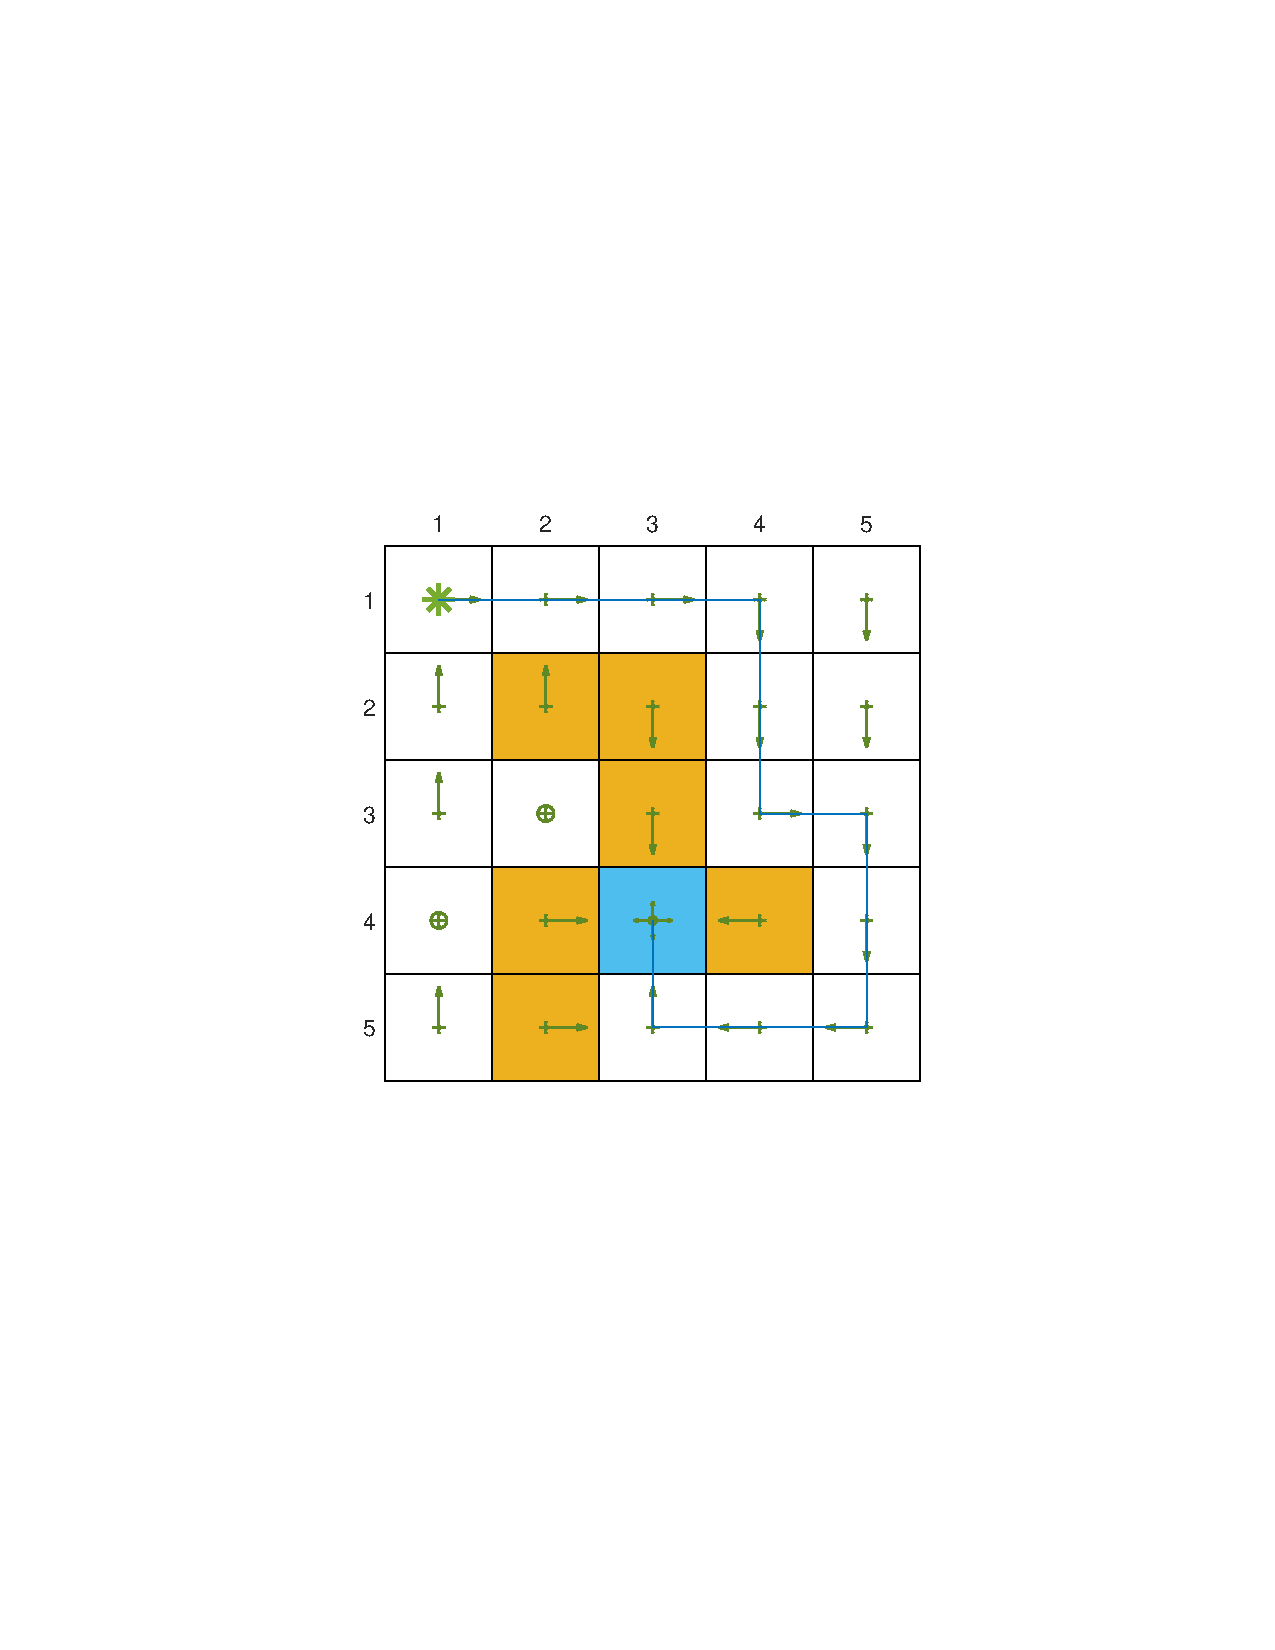
\includegraphics[width=0.29\linewidth]{fig_SarsaLinear_fianlPolicy}
\end{figure}
For details, please see the book.
}

\end{frame}
%---------------------
\AtBeginSection[]% put it to the start of each section
{
  \begin{frame}
    \frametitle{Outline}
    \tableofcontents[currentsection]
  \end{frame}
}
\section{Q-learning with function approximation}
%---------------------
\begin{frame}
\frametitle{Q-learning with function approximation}

Similar to Sarsa, tabular Q-learning can also be extended to the case of value function approximation.

\pause
\vspace{20pt}
The q-value update rule is
{\small\red{
\begin{align*}%\label{chapterFA_eq_QlearningFA}
w_{t+1}
&=w_t+\alpha_t\Big[r_{t+1}+\gamma \max_{a\in\A(s_{t+1})}\hat{q}(s_{t+1},a,w_t)-\hat{q}(s_t,a_t,w_t)\Big]\nabla_w \hat{q}(s_t,a_t,w_t),
\end{align*}}}
which is the same as Sarsa except that $\hat{q}(s_{t+1},a_{t+1},w_t)$ is replaced by $\max_{a\in\A(s_{t+1})}\hat{q}(s_{t+1},a,w_t)$.

\end{frame}
%---------------------
\begin{frame}
\frametitle{Q-learning with function approximation}

\begin{figure}[]
{\footnotesize
\begin{mdframed}[style=myAlgo,nobreak=true,frametitle={Pseudocode: Q-learning with function approximation (on-policy version)}]
{\fontfamily{cmss}\selectfont
\textbf{Initialization:}
Initial parameter $w_0$. Initial policy $\pi_0$.
$\alpha_t=\alpha>0$ for all $t$. $\epsilon\in(0,1)$.

\textbf{Goal:} Learn an optimal path to lead the agent to the target state from an initial state $s_0$.

\vspace{5pt}
For each episode, do

\qquad If $s_t$ ($t=0,1,2,\dots$) is not the target state, do

\setlength{\leftskip}{4em}
Collect the experience sample $(a_t,r_{t+1},s_{t+1})$ given $s_t$: generate $a_t$ following $\pi_t(s_t)$; generate $r_{t+1},s_{t+1}$ by interacting with the environment.

\setlength{\leftskip}{0em}

\qquad\qquad \blue{Update value (update parameter):}

\setlength{\leftskip}{4em} 
$w_{t+1}
=w_t+\alpha_t\Big[r_{t+1}+\gamma \max_{a\in\A(s_{t+1})}\hat{q}(s_{t+1},a,w_t)-\hat{q}(s_t,a_t,w_t)\Big]\nabla_w \hat{q}(s_t,a_t,w_t)$

\setlength{\leftskip}{4em} \blue{Update policy:}

\setlength{\leftskip}{4em} $\pi_{t+1}(a|s_t)=1-\frac{\varepsilon}{|\A(s_t)|}(|\A(s_t)|-1)$ if $a=\arg\max_{a\in\A(s_t)} \hat{q}(s_t,a,w_{t+1})$

\qquad\qquad $\pi_{t+1}(a|s_t)=\frac{\varepsilon}{|\A(s_t)|}$ otherwise
}%font
\end{mdframed}
}
\end{figure}
\end{frame}
%---------------------
\begin{frame}
\frametitle{Q-learning with function approximation}
Illustrative example:
\begin{itemize}
\item Q-learning with \blue{linear function} approximation: $\hat{q}(s,a,w)=\phi^T(s,a)w$
\item $\gamma=0.9$, $\epsilon=0.1$, $r_{\rm boundary}=r_{\rm forbidden}=-10$, $r_{\rm target}=1$, $\alpha=0.001$.
\end{itemize}
\begin{figure}[h]
\centering
\includegraphics[width=0.4\linewidth]{fig_QlearningLinear_rewardLength}\qquad
\includegraphics[width=0.29\linewidth]{fig_QlearningLinear_fianlPolicy}
\end{figure}
\end{frame}
%---------------------
\AtBeginSection[]% put it to the start of each section
{
  \begin{frame}
    \frametitle{Outline}
    \tableofcontents[currentsection]
  \end{frame}
}
\section{Deep Q-learning}
%---------------------
\begin{frame}
\frametitle{Deep Q-learning}

\blue{Deep Q-learning} or \blue{deep Q-network} (DQN):
\begin{itemize}
\pause
\item
One of the earliest and most successful algorithms that introduce deep neural networks into RL.
\pause
\item The role of neural networks is to be a nonlinear function approximator.
\pause
\item Different from the following algorithm:
{\small
\begin{align*}%\label{chapterFA_eq_QlearningFA}
w_{t+1}
&=w_t+\alpha_t\Big[r_{t+1}+\gamma \max_{a\in\A(s_{t+1})}\hat{q}(s_{t+1},a,w_t)-\hat{q}(s_t,a_t,w_t)\Big]\nabla_w \hat{q}(s_t,a_t,w_t)
\end{align*}
}
because of the way of training a network.
\end{itemize}

\end{frame}
%---------------------
\begin{frame}
\frametitle{Deep Q-learning}
Deep Q-learning aims to minimize the objective function/loss function:
\begin{align*}%\label{chapterFA_eq_objFcnQlearning}
w_{t+1}
=&w_t+\alpha_t\Big[\red{r_{t+1}+\gamma \max_{a\in\A(s_{t+1})}\hat{q}(s_{t+1},a,w_t)-\hat{q}(s_t,a_t,w_t)}\Big]\nabla_w \hat{q}(s_t,a_t,w_t)\\
&\qquad\qquad\qquad\qquad\qquad\qquad\red{\Downarrow}\\
&J(w)=\E\left[\left(\red{R+\gamma \max_{a\in\A(S')}\hat{q}(S',a,w)-\hat{q}(S,A,w)}\right)^2\right]
\end{align*}
where $(S,A,R,S')$ are random variables.
%\pause
%\begin{itemize}
%\item
%This corresponds to the \blue{Bellman optimality error}. That is because
%\begin{align*}%\label{eq_qlearningSolvingEquation}
%q(s,a)=\E\left[R_{t+1}+\gamma\max_{a\in\A(S_{t+1})}q(S_{t+1},a)\Big|S_t=s,A_t=a\right],\quad\forall s,a
%\end{align*}
%The value of
%$$R+\gamma \max_{a\in\A(S')}\hat{q}(S',a,w)-\hat{q}(S,A,w)$$ should be zero in the expectation sense
%\end{itemize}
\end{frame}
%---------------------
\begin{frame}
\frametitle{Deep Q-learning}
How to minimize the objective function? Gradient-descent!
\begin{itemize}
\pause
\item How to calculate the gradient of the objective function? Tricky!
\pause
\item That is because, in this objective function
\begin{align*}%\label{chapterFA_eq_objFcnQlearning}
J(w)=\E\left[\left(R+\gamma \max_{a\in\A(S')}\hat{q}(S',a,w)-\hat{q}(S,A,w)\right)^2\right],
\end{align*}
the parameter $w$ not only appears in $\hat{q}(S,A,w)$ but also in
$$y\doteq R+\gamma \max_{a\in\A(S')}\hat{q}(S',a,w)$$

\pause
\item Since the optimal $a$ depends on $w$,
$$\nabla_w y\ \red{\ne} \ \gamma \max_{a\in\A(S')}\nabla_w \hat{q}(S',a,w)$$

\pause
\item
To solve this problem, we can assume that $w$ in $y$ is fixed (at least for a while) when we calculate the gradient.
\end{itemize}

\end{frame}
%---------------------
\begin{frame}
\frametitle{Deep Q-learning}
To do that, we can introduce two networks.
\begin{itemize}
\pause
\item One is a \blue{main network} representing $\hat{q}(s,a,w)$
\item The other is a \blue{target network} $\hat{q}(s,a,w_T)$.
\end{itemize}
\pause
The objective function in this case degenerates to
$$J=\E\left[\left(R+\gamma \max_{a\in\A(S')}\red{\hat{q}(S',a,w_T)}-\blue{\hat{q}(S,A,w)}\right)^2\right],$$
where $w_T$ is the target network parameter.

\pause
When $w_T$ is fixed, the gradient of $J$ can be easily obtained as
\begin{align*}%\label{chapterFA_eq_DQNGradient}
\nabla_w J=\E\left[\left(R+\gamma \max_{a\in\A(S')}\red{\hat{q}(S',a,w_T)}-\blue{\hat{q}(S,A,w)}\right)\blue{\nabla_w \hat{q}(S,A,w)} \right].
\end{align*}
\begin{itemize}
\pause
\item The \blue{basic idea} of deep Q-learning is to use the gradient-descent algorithm to minimize the objective function.
\pause
\item However, such an optimization process evolves some \blue{important techniques} that deserve special attention.
\end{itemize}
\end{frame}
%%---------------------
%\begin{frame}
%\frametitle{Deep Q-learning}
%When $w_T$ is fixed, the gradient of $J$ can be easily obtained as
%\begin{align*}%\label{chapterFA_eq_DQNGradient}
%\nabla_w J=\E\left[\left(R+\gamma \max_{a\in\A(S')}\red{\hat{q}(S',a,w_T)}-\blue{\hat{q}(S,A,w)}\right)\blue{\nabla_w \hat{q}(S,A,w)} \right].
%\end{align*}
%\begin{itemize}
%\pause
%\item The \blue{basic idea} of deep Q-learning is to use the gradient-descent algorithm to minimize the objective function.
%\pause
%\item However, such an optimization process evolves some \blue{important techniques} that deserve special attention.
%\end{itemize}
%\end{frame}
%---------------------
\begin{frame}
\frametitle{Deep Q-learning - Two networks}

\textbf{Technique 1:} \red{Two networks, a main network and a target network.}

\pause
\textbf{Why is it used?}
\begin{itemize}
\item The mathematical reason has been explained when we calculate the gradient.
\end{itemize}

\pause
\textbf{Implementation details:}
\begin{itemize}
\item
Let $w$ and $w_T$ denote the parameters of the main and target networks, respectively. They are set to be the same initially.
\pause
\item
In every iteration, we draw a mini-batch of samples $\{(s,a,r,s')\}$ from the replay buffer (will be explained later).
\pause
\item For every $(s,a,r,s')$, we can calculate the desired output as $$y_T\doteq r+\gamma \max_{a\in\A(s')}\hat{q}(s',a,w_T)$$
Therefore, we obtain a mini-batch of data:
\vspace{-5pt}
$$\{(s,a,y_T)\}$$

\pause
\vspace{-5pt}
\item Use $\{(s,a,y_T)\}$ to train the network so as to minimize $(y_T-\hat{q}(s,a,w))^2$.
\end{itemize}
\end{frame}
%---------------------
\begin{frame}
\frametitle{Deep Q-learning - Experience replay}
\textbf{Technique 2:} \red{Experience replay}

\pause
\textbf{Question:} What is experience replay?

\pause
\textbf{Answer:}
\begin{itemize}
\item After we have collected some experience samples, we do NOT use these samples \blue{in the order they were collected}.
\pause
\item Instead, we store them in a set, called \blue{replay buffer $\mathcal{B}\doteq\{(s,a,r,s')\}$}
\pause
\item Every time we train the neural network, we can \blue{draw a mini-batch} of random samples from the replay buffer.
\pause
\item The draw of samples, or called \blue{experience replay}, should follow a \blue{uniform distribution}.
\end{itemize}
\end{frame}
%---------------------
\begin{frame}
\frametitle{Deep Q-learning - Experience replay}

\textbf{Question:} Why is experience replay necessary in deep Q-learning? Why does the replay must follow a uniform distribution?

\pause
\textbf{Answer:} The answers lie in the objective function.
\begin{align*}%\label{chapterFA_eq_objFcnQlearning}
J=\E\left[\left(R+\gamma \max_{a\in\A(S')}\hat{q}(S',a,w)-\hat{q}(S,A,w)\right)^2\right]
\end{align*}
\begin{itemize}
\pause
\item \blue{$R\sim p(R|S,A), S'\sim p(S'|S,A)$}: $R$ and $S��$ are determined by the system model.
\pause
\item \blue{$(S,A)\sim d$}: $(S,A)$ is an index
\pause
\item The distribution of the state-action pair $(S,A)$ is assumed to be \blue{uniform}.
\pause
\begin{itemize}
\item[-] Why uniform distribution? Because no prior knowledge.
\item[-] Can we use stationary distribution like before? No, since no policy is given.
\end{itemize}
\end{itemize}
\end{frame}
%---------------------
\begin{frame}
\frametitle{Deep Q-learning - Experience replay}

\textbf{Answer (continued):}
\begin{itemize}
\item However, \blue{the samples are not uniformly collected} because they are generated consequently by certain policies.
\pause
\item To \blue{break the correlation} between consequent samples, we can use the experience replay technique by uniformly drawing samples from the replay buffer.
\pause
\item This is the \blue{mathematical reason} why experience replay is necessary and why the experience replay must be uniform.
\end{itemize}
\end{frame}
%---------------------
\begin{frame}
\frametitle{Deep Q-learning - Experience replay}
\textbf{Revisit the tabular case:}
\begin{itemize}
\pause
\item Question: Why does not tabular Q-learning require experience replay?
\pause
\begin{itemize}
\item[-] Answer: Because it does not require any distribution of $S$ or $A$.
\end{itemize}
\pause
\item Question: Why does Deep Q-learning involve distributions?
\pause
\begin{itemize}
\item[-] Answer: Because we need to define a \emph{scalar} objective function $J(w)=\E[*]$, where $\E$ is for all $(S,A)$.
\item[-] The tabular case aims to solve a set of equations for all $(s,a)$ (Bellman optimality equation), whereas the deep case aims to optimize a scalar objective function.
\end{itemize}
\pause
\item Question: Can we use experience replay in tabular Q-learning?
\pause
\begin{itemize}
\item[-] Answer: Yes, we can. And more sample efficient (why?)
\end{itemize}
\end{itemize}
\end{frame}
%---------------------
\begin{frame}
\frametitle{Deep Q-learning}
\vspace{-5pt}
{\footnotesize

\begin{figure}[]
\begin{mdframed}[style=myAlgo,nobreak=true,frametitle={Pseudocode: Deep Q-learning (off-policy version)}]
{\fontfamily{cmss}\selectfont

\textbf{Initialization:} A main network and a target network with the same initial parameter.

\textbf{Goal:} Learn an optimal target network to approximate the \emph{optimal} action values from the experience samples generated by a given behavior policy $\pi_b$.

\vspace{5pt}
Store the experience samples generated by $\pi_b$ in a replay buffer $\mathcal{B}=\{(s,a,r,s')\}$

\setlength{\leftskip}{2em}
For each iteration, do

\setlength{\leftskip}{4em} Uniformly draw a mini-batch of samples from $\mathcal{B}$

\setlength{\leftskip}{4em}
For each sample $(s,a,r,s')$, calculate the target value as $y_T=r+\gamma \max_{a\in\A(s')}\hat{q}(s',a,w_{T})$, where $w_{T}$ is the parameter of the target network

\setlength{\leftskip}{4em}
Update the main network to minimize $(y_T-\hat{q}(s,a,w))^2$ using the mini-batch of samples

\qquad
Set $w_T=w$ every $C$ iterations
}%font
\end{mdframed}
\end{figure}
\vspace{-5pt}
\pause
Remarks:
\begin{itemize}
\item Why no policy update?
\pause
\item The network input and output are different from the DQN paper.
\end{itemize}
}
\end{frame}
%---------------------
\begin{frame}
\frametitle{Deep Q-learning}
Illustrative example:
\begin{itemize}
\item We need to \blue{learn optimal action values for every state-action pair}.
\item Once the optimal action values are obtained, the optimal greedy policy can be obtained immediately.
\end{itemize}

\end{frame}
%---------------------
\begin{frame}
\frametitle{Deep Q-learning}

Setup:
\begin{itemize}
\pause
\item One single episode is used to train the network.
\pause
\item This episode is generated by an exploratory behavior policy shown in Fig.~(a).
\pause
\item The episode only has 1,000 steps! The tabular Q-learning requires 100,000 steps.
\pause
\item A shallow neural network with one single hidden layer is used as a nonlinear approximator of $\hat{q}(s,a,w)$. The hidden layer has 100 neurons.
\end{itemize}

\pause
See details in the book.

\end{frame}
%---------------------
\begin{frame}
\frametitle{Deep Q-learning}
\vspace{-30pt}
\captionsetup[subfigure]{labelformat=empty}
\begin{figure}[h]
\centering
\subfloat[The behavior policy.]{
\includegraphics[width=0.3\linewidth]{fig_QLearningOffPolicyNN_behavePolicy}}
\subfloat[An episode of 1,000 steps.]{\quad
\visible<2->{\includegraphics[width=0.3\linewidth]{fig_QLearningOffPolicyNN_episode_epiLenth1000}}\quad}
\subfloat[The obtained policy.]{
\visible<3->{\includegraphics[width=0.3\linewidth]{fig_QLearningOffPolicyNN_targetPolicy_epiLenth1000}}\quad}\\
\subfloat[The TD error converges to zero.]{\qquad
\visible<4->{\includegraphics[width=0.3\linewidth]{fig_QLearningOffPolicyNN_lossFcn_epiLenth1000}}\qquad}
\subfloat[The state estimation error converges to zero.]{\qquad\qquad
\visible<5->{\includegraphics[width=0.3\linewidth]{fig_QLearningOffPolicyNN_sValueError_epiLenth1000}}\qquad\qquad}
%\caption{Optimal policy searching by deep Q-learning. Here, $\gamma=0.9$, $r_{\rm boundary}=r_{\rm forbidden}=-10$, and $r_{\rm target}=1$. The batch size is 100.}
%\label{chapterFA_fig_exampleDeepQLearning1}
\end{figure}
\end{frame}
%---------------------
\begin{frame}
\frametitle{Deep Q-learning}
\textbf{What if we only use a single episode of 100 steps}? Insufficient data

\vspace{-20pt}
\begin{figure}[h]
\centering
\setcounter{subfigure}{0}
\captionsetup[subfigure]{labelformat=empty}
\subfloat[The behavior policy.]{
\includegraphics[width=0.3\linewidth]{fig_QLearningOffPolicyNN_behavePolicy}}
\subfloat[An episode of 100 steps.]{\quad
\visible<2->{\includegraphics[width=0.3\linewidth]{fig_QLearningOffPolicyNN_episode_epiLenth100}}\quad}
\subfloat[The final policy.]{
\visible<3->{\includegraphics[width=0.3\linewidth]{fig_QLearningOffPolicyNN_targetPolicy_epiLenth100}}\quad}\\
\subfloat[The TD error converges to zero.]{\qquad
\visible<4->{\includegraphics[width=0.3\linewidth]{fig_QLearningOffPolicyNN_lossFcn_epiLenth100}}\qquad}
\subfloat[The state error does not converge to zero.]{\qquad\qquad
\visible<5->{\includegraphics[width=0.3\linewidth]{fig_QLearningOffPolicyNN_sValueError_epiLenth100}}\qquad\qquad}
\end{figure}
\end{frame}
%--------------------------------------
\AtBeginSection[]% put it to the start of each section
{
  \begin{frame}
    \frametitle{Outline}
    \tableofcontents[currentsection]
  \end{frame}
}
\section{Summary}
%---------------------
\begin{frame}
\frametitle{Summary}

This lecture introduces the method of value function approximation.
\begin{itemize}
\item First, understand the basic idea.
\item Second, understand the basic algorithms.
\end{itemize}

\end{frame}
%---------------------
%%%%%%%%%%%%%%%%%%%%%%%%%%%%%%%%%%%%%%%%%%%%%%%%%%%%%%%%%%%%%%%%%%%%%%%%%%%%%%%%%%%%%%%%%%%%%%%%%%
%\bibliographystyle{plainnat}
%\bibliography{myOwnPub,zsyReferenceAll}
\end{document}
